\section{Thurstonian Ranking Model} \label{sec::tpp_trm}

The original Thurstonian ranking model (\textsc{Trm})~\cite{thurstone1927law} is
devised for analyzing ordinal data.  Suppose in a ranking annotation task, $K$
workers $\{t_k\}_{k=1}^{K}$ are given $Q$ queries $\{q_l\}_{l=1}^Q$ and $D$
documents $\{d_i\}_{i=1}^D$.  It is postulated that the optimal ranked
list\footnote{a permutation of documents} for query $q_l$ is determined by the
\emph{ground truth relevance score} $s_{l,i}$ of each document $d_i$.
Precisely, the larger the value of $s_{l,i}$, the higher rank is assigned to
$d_i$.  Each worker $t_k$ produces a ranked list $\sigma_l^{(k)}$ by ordering
documents according to his \emph{perceived relevance scores} $s_{l,i}^{(k)}$,
which are assumed to be Gaussian distributed: $s_{l,i}^{(k)} \sim
\mathrm{N}(s_{l,i}, \delta_l^2)$.  The variance $\delta_l^2$ quantifies the
\emph{query difficulty} of $q_l$: $\delta_l^2$ is larger for more difficult
query, and the perceived score can deviate more from the ground truth score.

\begin{figure}[h!]
	\begin{center}
		\includegraphics[width=0.4\textwidth]{crowd-thurstonian/figure/thurstonian.png}
		\caption{Plate notation for \textsc{Trm}} \label{fig::thurstonian}
		\includegraphics[width=0.5\textwidth]{crowd-thurstonian/figure/tpp.png}
		\caption{Plate notation for \textsc{Tpp}} \label{fig::tpp}
	\end{center}
\end{figure}

The plate notation of the above generative process is given in
\Cref{fig::thurstonian}.  With the workers' annotated rankings
$\{\sigma_l^{(k)}\}$ given as observations, the goal of \textsc{Trm} is to infer
$\{s_{l,i}\}$ as well as $\{\delta_l^2\}$.  Algorithmic development for
inference previously investigated includes maximum likelihood
estimation~\cite{bockenholt1993applications} and Bayesian
inference~\cite{yao1999bayesian}. A derivation of the maximum likelihood
estimation is given in \Cref{app::trm}.

\section{Thurstonian Pairwise Preference} \label{sec::tpp_tpp}

\begin{table}[h!]
\caption{Summary of Notations} \label{tab::tpp_notation}
\begin{center}
\begin{tabular}{ll}
\hline
Notation 	& Explanation \\
\hline
\hline
$t_k$, $q_l$, $d_i$					&
      worker $t_k$, query $q_l$ and document $d_i$ \\
$s_{l,i}$  							    &
      ground truth relevance score of $d_i$ \emph{w.r.t.} $q_l$\\
$\delta_l^2$ 						    &
      the difficulty of query $q_l$\\
$m_l$								        &
      the domain of query $q_l$ \\
\multirow{2}{*}{$\vect{\theta}=(\theta_1, \dots ,\theta_M)^T$}		&
      the distribution of query domains,      \\                  &
      $m_l \sim \mathrm{Mult}(\vect{\theta})$ \\
\multirow{2}{*}{$\tau_{k,m}$}		                                  &
      worker $t_k$'s expertise \& truthfulness \\                 &
      on domain $m$\\
$s_{l,i}^{(k)}$ 						&
      worker $t_k$'s perceived score of $d_i$ \emph{w.r.t.} $q_l$\\
\multirow{2}{*}{$\pi=\langle k,l,i_1,i_2 \rangle$} 	              &
      pairwise preference $\pi$: $t_k$ prefers document \\        &
      $d_{i_1}$ to document $d_{i_2}$ \emph{w.r.t.} $q_l$\\
\multirow{2}{*}{$\tilde{s}_{i_1}^{\pi}, \tilde{s}_{i_2}^{\pi}$}	  &
      noisy scores of $d_{i_1}$ and $d_{i_2}$ to determine \\     &
      pairwise preference $\pi$\\
$\Delta s^{\pi}$ 					                                        &
      noisy score difference
      $\Delta s^{\pi} = \tilde{s}_{i_1}^{\pi} - \tilde{s}_{i_2}^{\pi}$  \\
$\mathbf{\Theta} = \{ s_{l,i}, \delta_l^2, \theta_m, \tau_{k,m}\}$ 	&
      model parameters \\
$\mathbf{Z} = \{m_l, s_{l,i}^{(k)}\}$ 							              	&
      latent variables of interest \\
$\mathbf{V} = \{\Delta s^{\pi}\}$									                  &
      auxiliary latent variables \\
$\mathbf{D} = \{\pi\}$											                        &
      observations \\
\hline
\end{tabular}
\end{center}
\end{table}%

\trm{}  specifies the generation of ranked lists in a crowdsourced setting, with
variable query difficulty taken into account. However, the difficulty in
obtaining annotated \emph{ranked lists} makes it hardly applicable in practice.
We propose a novel generative model called ``Thurstonian Pairwise Preference''
(\tpp{}), which extends \trm{} to accommodate \emph{pairwise preferences} as
observations. Meanwhile, \tpp{} seamlessly integrates a \emph{worker-aware}
layer with the original query-aware layer to incorporate workers' variable
expertise across different domains and their truthfulness, which explains the
generation of the inconsistent pairwise preferences at modeling time.

The plate notation of \textsc{Tpp} is given in \Cref{fig::tpp}. The
notations used throughout this chapter are summarized in
\Cref{tab::tpp_notation}. Suppose worker $t_k$ compares documents $d_{i_1}$ and
$d_{i_2}$ \emph{w.r.t.} query $q_l$. The pairwise preference $\pi$ is either
$t_k$ prefers $d_{i_1}$ to $d_{i_2}$, denoted by $\langle k, l, i_1, i_2
\rangle$, or $\pi = \langle k, l, i_2, i_1 \rangle$ if $t_k$ prefers
$d_{i_2}$\footnote{We adopt the assumption made in \trm{} that no ties exist in
rankings. However, if two documents are indeed equally relevant, the workers
shall randomly prefers either one, and the ground truth relevance scores of
the two documents would be close.}. The preference depends on query
difficulty, as well as the domain expertise and truthfulness of the worker.

\tpp{} first generates the workers' perceived scores in the same way as \trm{}
does. Then it introduces a worker-aware layer to simulate the generation of
pairwise annotations, which involves a delicate modeling of query domains.  We
assume there are $M$ domains. For query $q_l$, its domain $m_l$ is drawn from a
multinomial distribution: $m_l \sim \mathrm{Mult}(\vect{\theta})$. In order to
generate the pairwise preference $\pi$, worker $t_k$ generates two noisy scores
$\tilde{s}_{i_1}^{\pi}$ and $\tilde{s}_{i_2}^\pi$, which are Guassian
distributed: $\tilde{s}_{i_1}^{\pi} \sim \mathrm{N}(\mathrm{sgn}(\tau_{k,m_l})
  s_{l,i_1}^{(k)}, \tau_{k,m_l}^{-2})$ and $\tilde{s}_{i_2}^{\pi} \sim
  \mathrm{N}(\mathrm{sgn}(\tau_{k,m_l}) s_{l,i_2}^{(k)},
\tau_{k,m_l}^{-2})$.\footnote{$\mathrm{sgn}(x) =\left\{  \begin{array}{ll} 1 &
\textrm{if}~x > 0 \\ -1 & \textrm{otherwise}\end{array} \right.$} The parameter
$\tau_{k,m}$ encodes worker $t_k$'s expertise and truthfulness on domain $m$.
Specifically, the sign of $\tau_{k,m}$ indicates whether worker $t_k$ is
truthful or malicious on domain $m$. A malicious worker would have a negative
$\tau_{k,m}$, giving false preferences by ``flipping'' his perceived scores.
The absolute value of $\tau_{k,m}$ measures the expertise of $t_k$ on $m$: a
larger $|\tau_{k,m}|$ means a smaller variance of the noisy score, \ie, $t_k$ is
more knowledgeable on $m$; for a very small $|\tau_{k,m}|$, the noisy score is
nearly uniformly distributed, implying $t_k$ likely to be a spammer. Given the
noisy scores $\tilde{s}_{i_1}^{\pi}$ and $\tilde{s}_{i_2}^\pi$, the pairwise
preference is uniquely determined: $\pi = \langle k, l, i_1, i_2 \rangle$ if
$\tilde{s}_{i_1}^{\pi} - \tilde{s}_{i_2}^{\pi}  \geq 0$ and vice versa.  We
define the \emph{noisy score difference} in this case as:
\begin{equation}
\Delta s^\pi =  \tilde{s}_{i_1}^{\pi} - \tilde{s}_{i_2}^{\pi}
\label{eq::tpp_deltas}
\end{equation}
and thus $\P(\pi = \langle k, l, i_1, i_2 \rangle) = \P(\Delta s^\pi \geq 0)$.

The generative process of \textsc{Tpp} is summarized as follows:

\begin{itemize}
\item \textbf{Generate Perceived Scores:} Generate worker $t_k$'s perceived
  score of document $d_i$ \emph{w.r.t.} query $q_l$:  $s_{l,i}^{(k)} \sim
  \mathrm{N}(s_{l,i}, \delta_l^2)$
\item \textbf{Generate Query Domains:} For query $q_l$, draw its domain: $m_l
  \sim \mathrm{Mult}(\vect{\theta})$.
\item \textbf{Generate Noisy Scores:} To compare two documents $d_{i_1}$ and
  $d_{i_2}$, worker $t_k$ generate noisy scores $\tilde{s}_{i_1}^{\pi}$ and
  $\tilde{s}_{i_2}^{\pi}$.
    \begin{equation}
    \tilde{s}_{i_j}^{\pi} \sim \mathrm{N}(
                        \mathrm{sgn}(\tau_{k,m_l}) s_{l,i_j}^{(k)},
                        \tau_{k,m_l}^{-2}) ~(j=1,2)
                        \label{eq::tpp_ns_gen}
    \end{equation}
\item \textbf{Generate Pairwise Preferences:} The pairwise preference $\pi$ is
  determined by the noisy score difference: $\pi=\langle k, l, i_1, i_2 \rangle$
  if $\Delta s^\pi  = \tilde{s}_{i_1}^{\pi} - \tilde{s}_{i_2}^{\pi}  \geq 0$,
  and $\pi=\langle k, l, i_2, i_1 \rangle$ if $\Delta s^\pi < 0$.
\end{itemize}

\begin{figure}[h!]
  \hspace{2.5cm}
		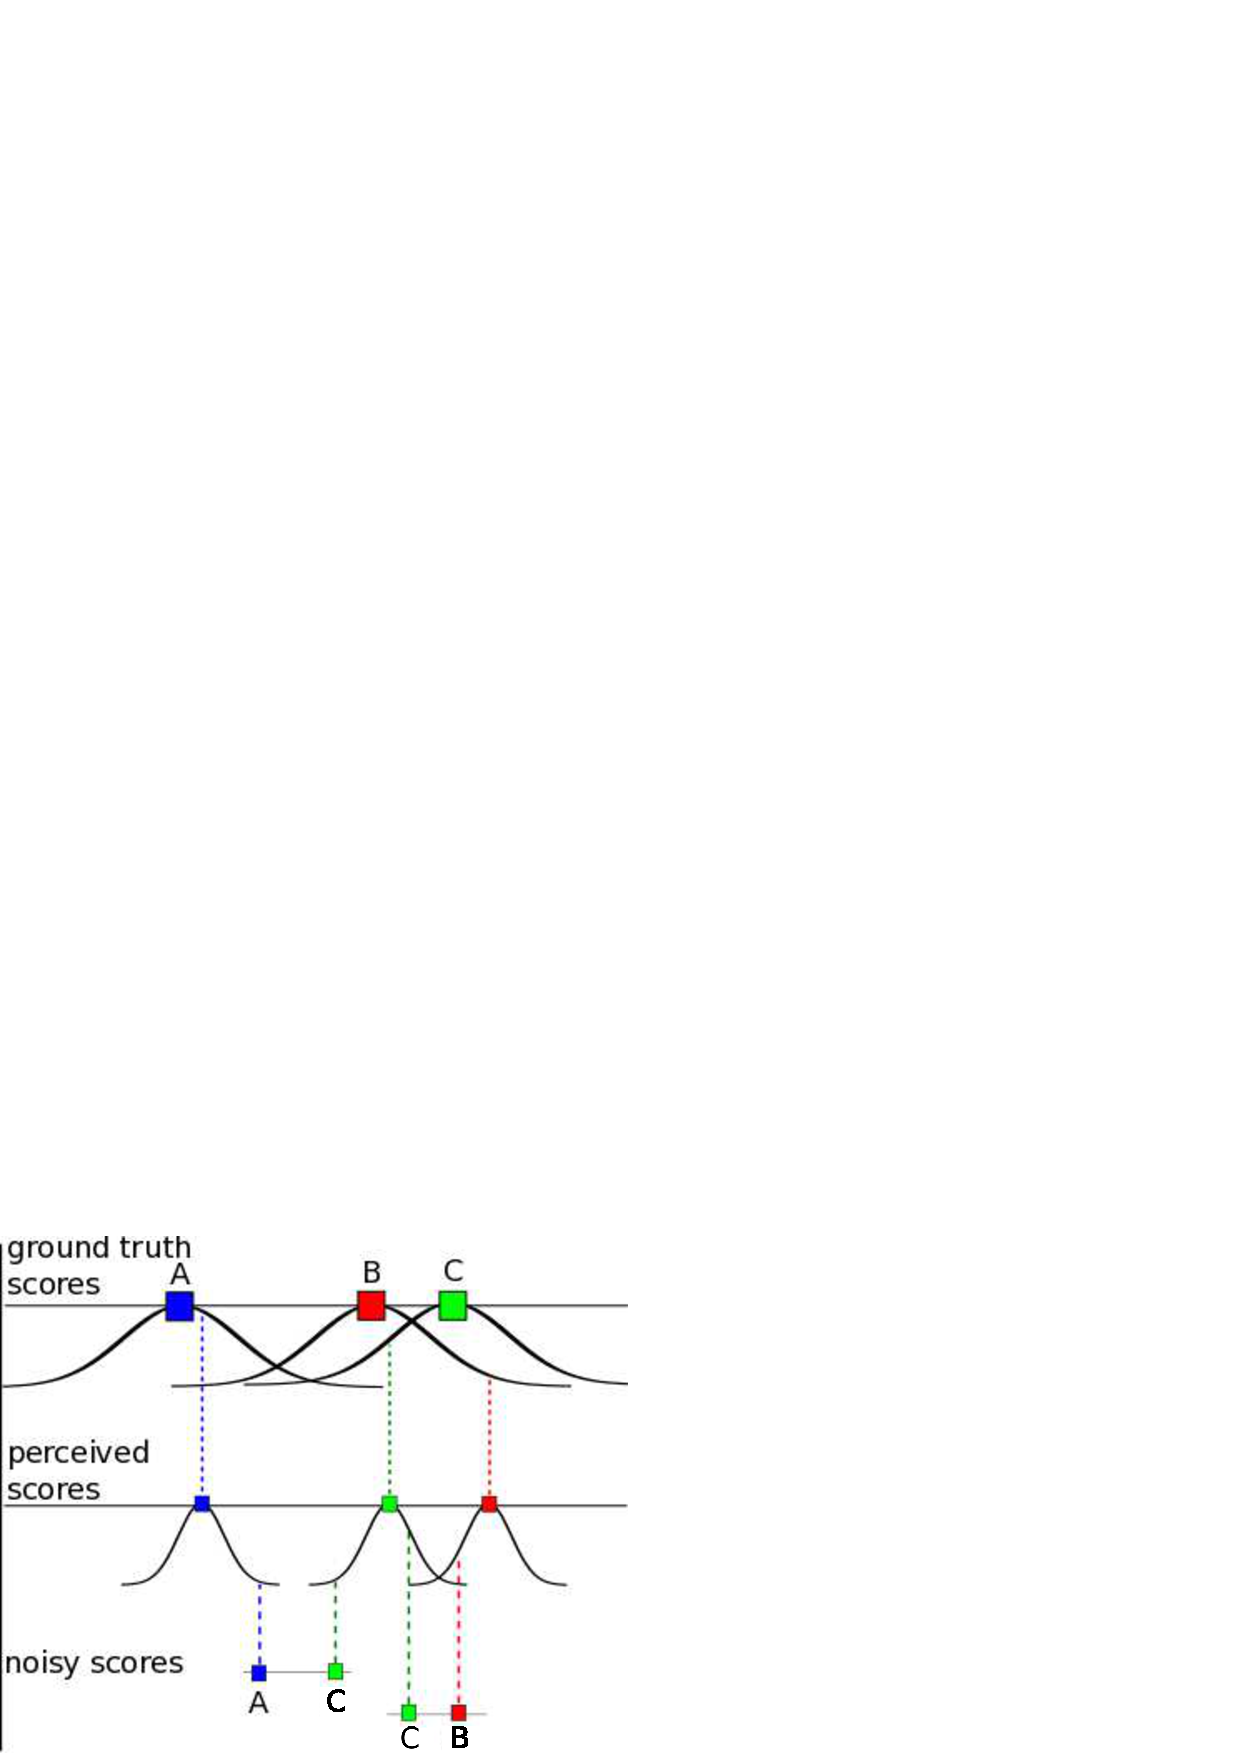
\includegraphics[scale=0.8,trim={0 14cm 0 6cm},clip]{crowd-thurstonian/figure/gaussian.pdf}
    \caption{An Illustration Example of \tpp{}: The generation of two pairwise
    preferences by a crowd worker for a given query} \label{fig::gaussian}
    \caption*{The true ranking is determined by the  ground truth scores of each
      document. The perceived score of each document is Gaussian distributed
      based on the true score and the query difficulty. Each time a worker is
      asked to compare a pair of documents, The perceived scores, together with
      the domain expertise and truthfulness of the worker, specify another two
      Gaussian distributions from which the noisy scores are drawn. The pairwise
      preference is given accordingly. The worker is truthful in this example.}
\end{figure}

\Cref{fig::gaussian} illustrates the generation of two pairwise
preferences by a crowd worker for a given query. The ground truth scores for
three documents $A,B,C$ imply the true ranking to be $A \prec B \prec C$. The
worker's perceived scores deviate from the ground truth scores due to query
difficulty. In fact, the perceived scores imply $A \prec C \prec B$, which
contradicts with the true ranking.  We further assume that the worker is
truthful and has reasonable domain knowledge (This example does not include the
generation of query domains for the sake of clarity). The worker generates noisy
scores which are close to his perceived scores, and gives pairwise
preferences~($A \prec C$, $C \prec B$) accordingly.  It is worth noting that a
pair of noisy scores are drawn each time a worker judges a pair of documents.
Thus \textsc{Tpp} respects {intra-worker inconsistency} as well as {inter-worker
inconsistency}.

